\documentclass[a4paper,12pt]{article}

\usepackage[utf8]{inputenc}
\usepackage{amsmath}
\usepackage{amsfonts}
\usepackage{amssymb}
\usepackage{graphicx}
\usepackage{hyperref}
\usepackage{geometry}
\geometry{a4paper, margin=1in}

\title{Overfitting and Regularisation, practical session notes}
\author{Noé Debrois}
\date{\today}

\begin{document}

\maketitle

\tableofcontents

\section{Early Stopping}

Overfitting networks show a monotonely-decreasing $\textit{training error}$ with the number of gradient descent iterations $k$. But they lose $\textbf{generalization}$ at some point.\\

So the idea is to hold out some data for validation, and while we train on the training set, we perform cross-validation on the (hold-out) validation set (i.e. you do 1 epoch of training and then you check the validation error). Training is stopped when the validation error increases.\\

Below, we can see how to create the EarlyStopping callback :

\begin{verbatim}
tf.keras.callbacks.EarlyStopping(
    monitor="val_loss",
    min_delta=0,
    patience=0,
    verbose=0,
    mode="auto",
    baseline=None,
    restore_best_weights=False,
    start_from_epoch=0)
\end{verbatim}

And here is how to include it in the $es\_model.fit()$. 

\begin{verbatim}
import tensorflow as tf
from tensorflow import keras as tfk

# Define the patience value for early stopping
patience = 100

# Create an EarlyStopping callback
early_stopping = tfk.callbacks.EarlyStopping(
    monitor='val_mse',
    mode='min',
    patience=patience,
    restore_best_weights=True)

# Store the callback in a list
callbacks = [early_stopping]

# Train the model and store the training history
es_history = es_model.fit(
    x = X_train,
    y = y_train,
    validation_data = (X_val, y_val),
    batch_size = batch_size,
    epochs = epochs,
    callbacks = callbacks).history
\end{verbatim}

Here is what we observe when we use EarlyStopping \ref{fig:early_stopping} :

\begin{figure}[h!]
    \centering
    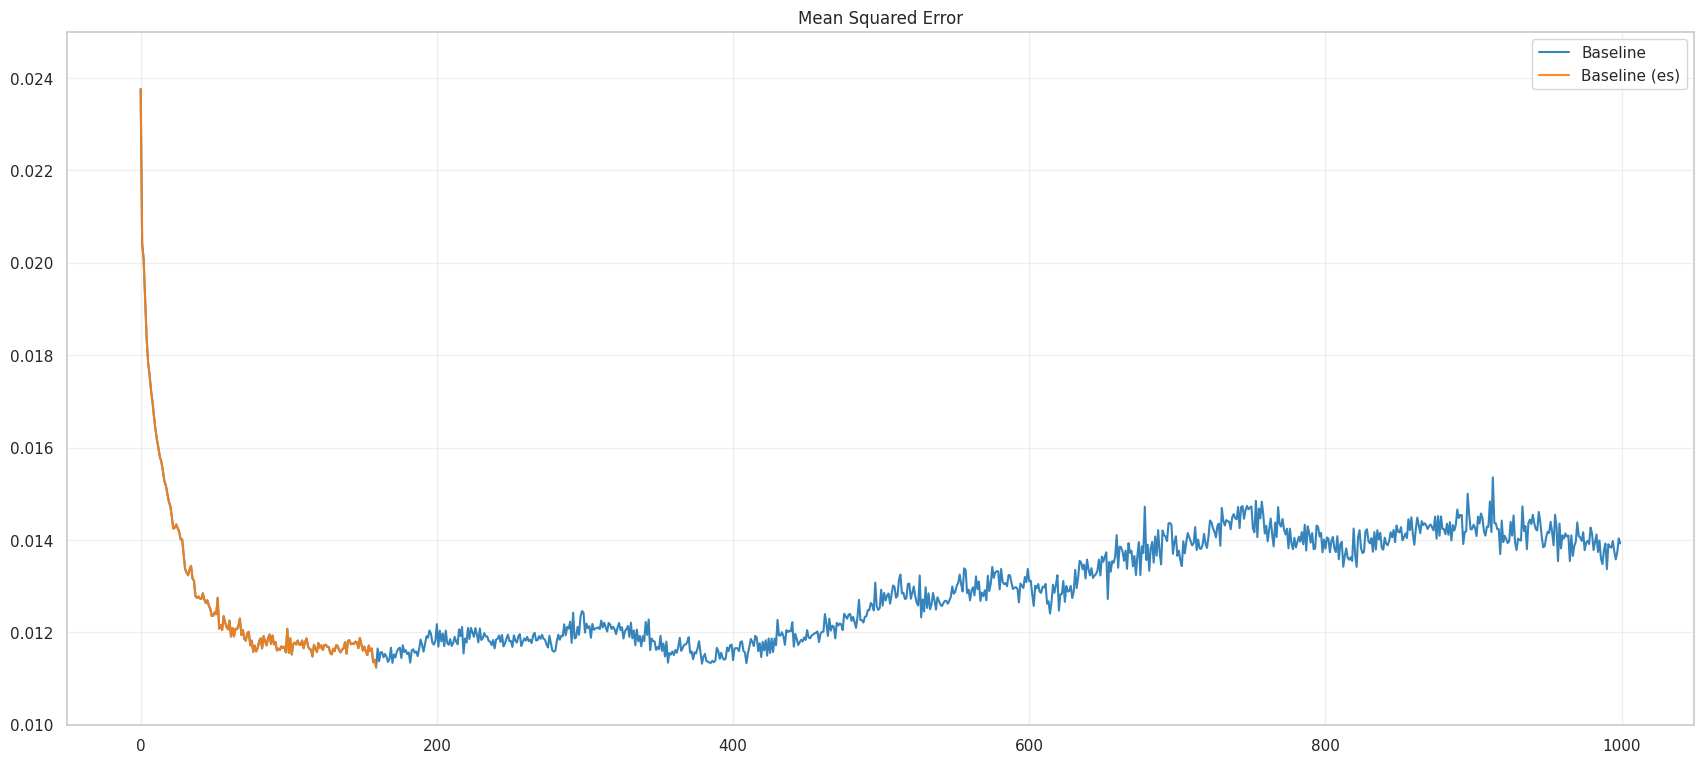
\includegraphics[width=1\textwidth]{EarlyStopping.png}
    \caption{Early stopping with patience = 100}
    \label{fig:early_stopping}
\end{figure}

\section{Regularisation}
\subsection{Ridge Regularisation}

Ridge regularisation is a L2 regularisation. It adds a term to the loss function that penalises large weights. The loss function becomes :
$$\mathrm{Ridge} (y, \hat{y}) = \frac{1}{N} \sum^N_{n=0} (y_n - g(x_n|w))^2 + \lambda\sum^K_{k=0}w_k^2 = \mathrm{MSE} (y, \hat{y}) + \lambda||w||_2^2$$\\

Here is how we can implement Ridge regularisation in a model using tensorflow keras (here we also implemented early stopping) :
\begin{verbatim}
l2_lambda = 5e-4
l2_model.summary(expand_nested=True, show_trainable=True)
l2_model = build_model(input_shape, l2_lambda=l2_lambda)
tfk.utils.plot_model(l2_model, expand_nested=True, show_trainable=True, show_shapes=True, dpi=70)

# Create an EarlyStopping callback
early_stopping = tfk.callbacks.EarlyStopping(
    monitor='val_mse',
    mode='min',
    patience=patience,
    restore_best_weights=True)

# Store the callback in a list
callbacks = [early_stopping]

# Train the model and store the training history
l2_history = l2_model.fit(
    x = X_train,
    y = y_train,
    validation_data = (X_val, y_val),
    batch_size = batch_size,
    epochs = epochs,
    callbacks = callbacks).history
\end{verbatim}

Here is what we observe when we use Ridge regularisation \ref{fig:ridge_regression} :

\begin{figure}[h!]
    \centering
    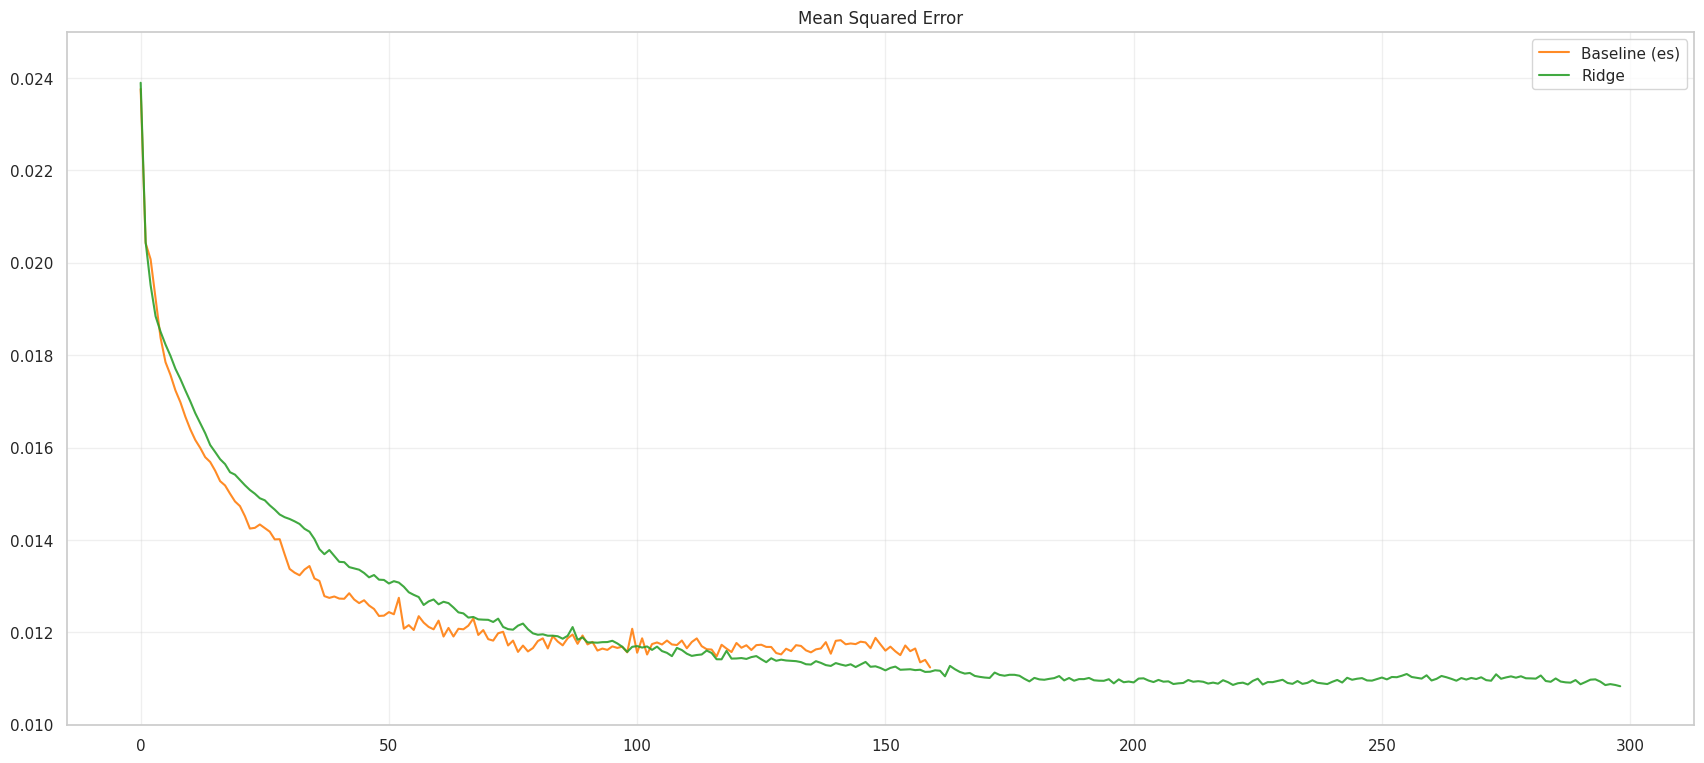
\includegraphics[width=1\textwidth]{RidgeRegression.png}
    \caption{Ridge regression with $\lambda = 5e-4$}
    \label{fig:ridge_regression}
\end{figure}

\subsection{Lasso Regularisation}
[To be completed]

\section{Dropout}
The Dropout layer randomly sets input units to 0 with a frequency of rate at each step during training time, which helps prevent overfitting. Inputs not set to 0 are scaled up by 1/(1 - rate) such that the sum over all inputs is unchanged.\\

Note that the Dropout layer only applies when training is set to True such that no values are dropped during inference.\\

Here is how we can implement Dropout in a model using tensorflow keras :

\begin{verbatim}
    tf.keras.layers.Dropout(
    rate,
    noise_shape=None,
    seed=None,
    **kwargs)
\end{verbatim}

Here is an example from exercise session 2 where we use Dropout and also EarlyStopping :

\begin{verbatim}
dropout_rate = 1/2
dropout_model = build_model(input_shape, dropout_rate=dropout_rate)
dropout_model.summary(expand_nested=True, show_trainable=True)
tfk.utils.plot_model(dropout_model, expand_nested=True, show_trainable=True, show_shapes=True, dpi=70)

# Create an EarlyStopping callback
early_stopping = tfk.callbacks.EarlyStopping(
    monitor='val_mse',
    mode='min',
    patience=patience,
    restore_best_weights=True)

callbacks = [early_stopping]

dropout_history = dropout_model.fit(
    x = X_train,
    y = y_train,
    validation_data = (X_val, y_val),
    batch_size = batch_size,
    epochs = epochs,
    callbacks = callbacks).history
\end{verbatim}

Here is what we observe when we use Dropout \ref{fig:dropout} :

\begin{figure}[h!]
    \centering
    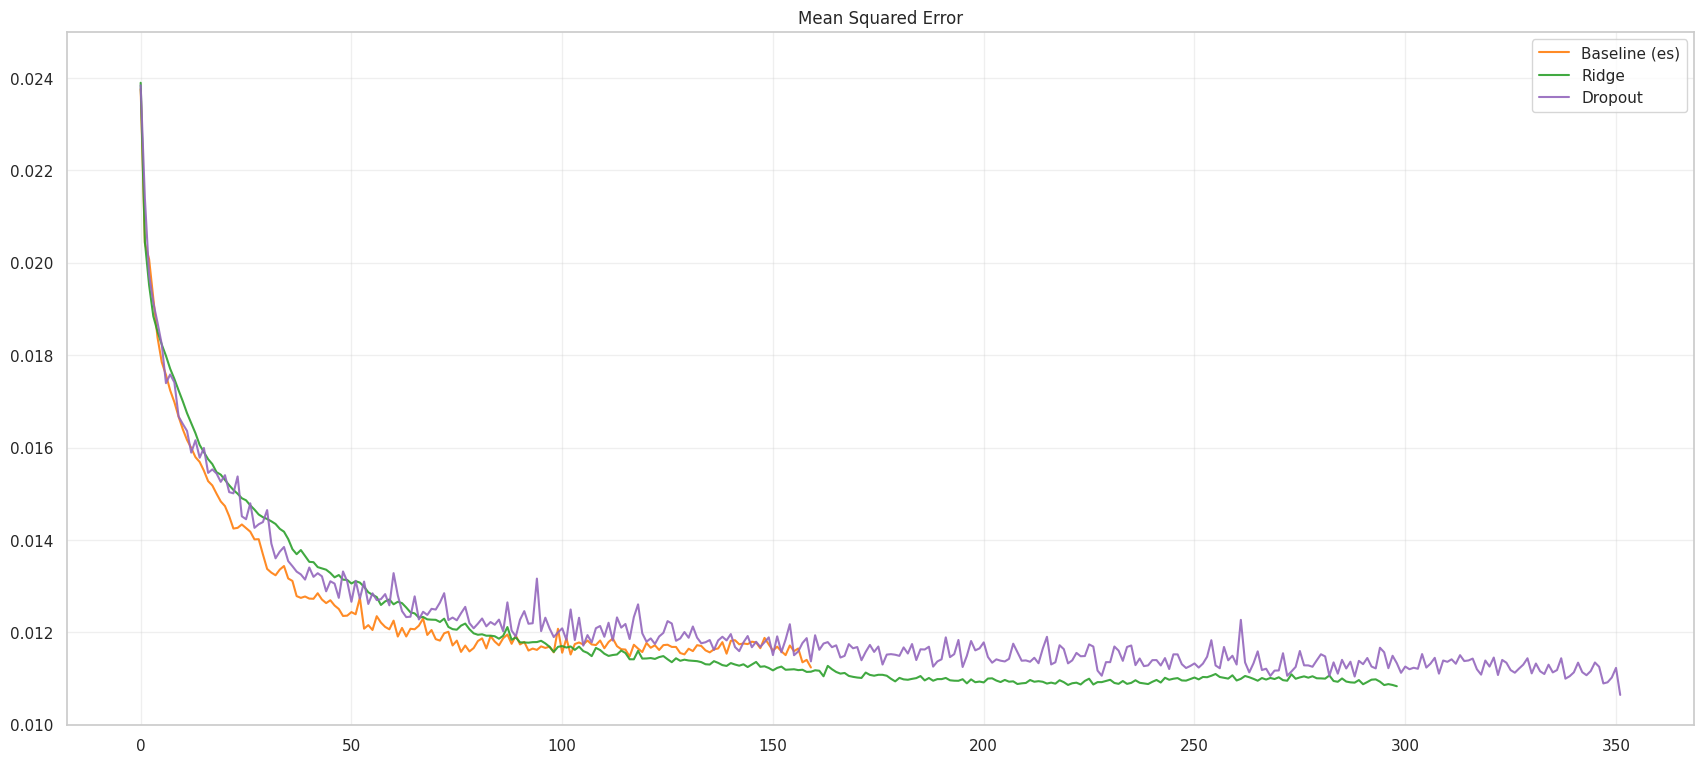
\includegraphics[width=1\textwidth]{Dropout.png}
    \caption{Dropout with rate = 1/2}
    \label{fig:dropout}
\end{figure}    

\section{Final Comparison of all methods}

The following figures come from the exercise session 2. For the regularisation method, only the Ridge one was implemented.

\begin{figure}[h!]
    \centering
    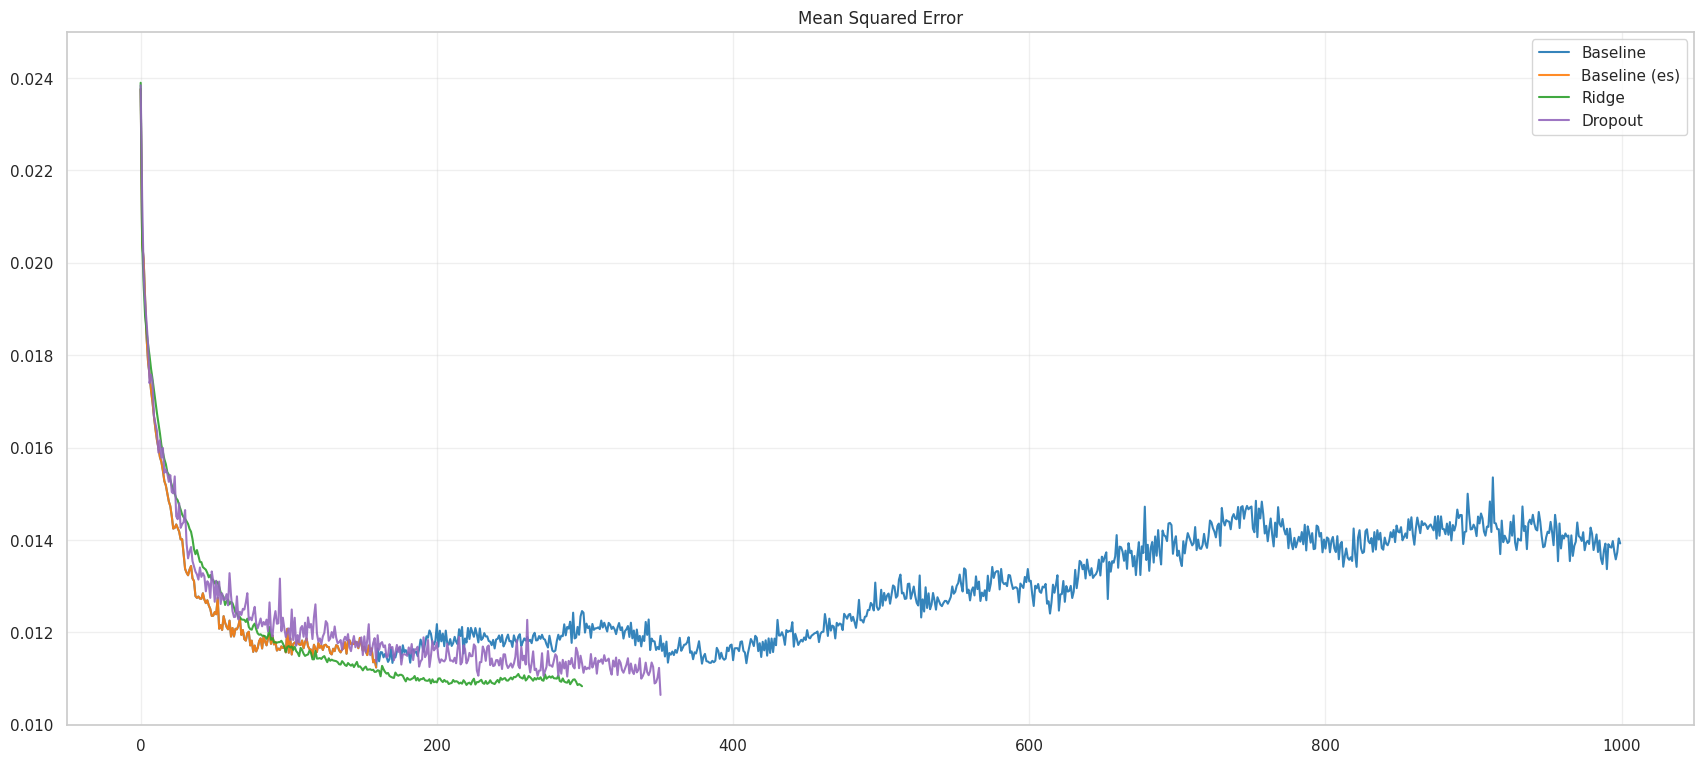
\includegraphics[width=1\textwidth]{Comparison1.png}
    \caption{Comparison of all methods}
    \label{fig:comparison}
\end{figure}    

\begin{figure}[h!]
    \centering
    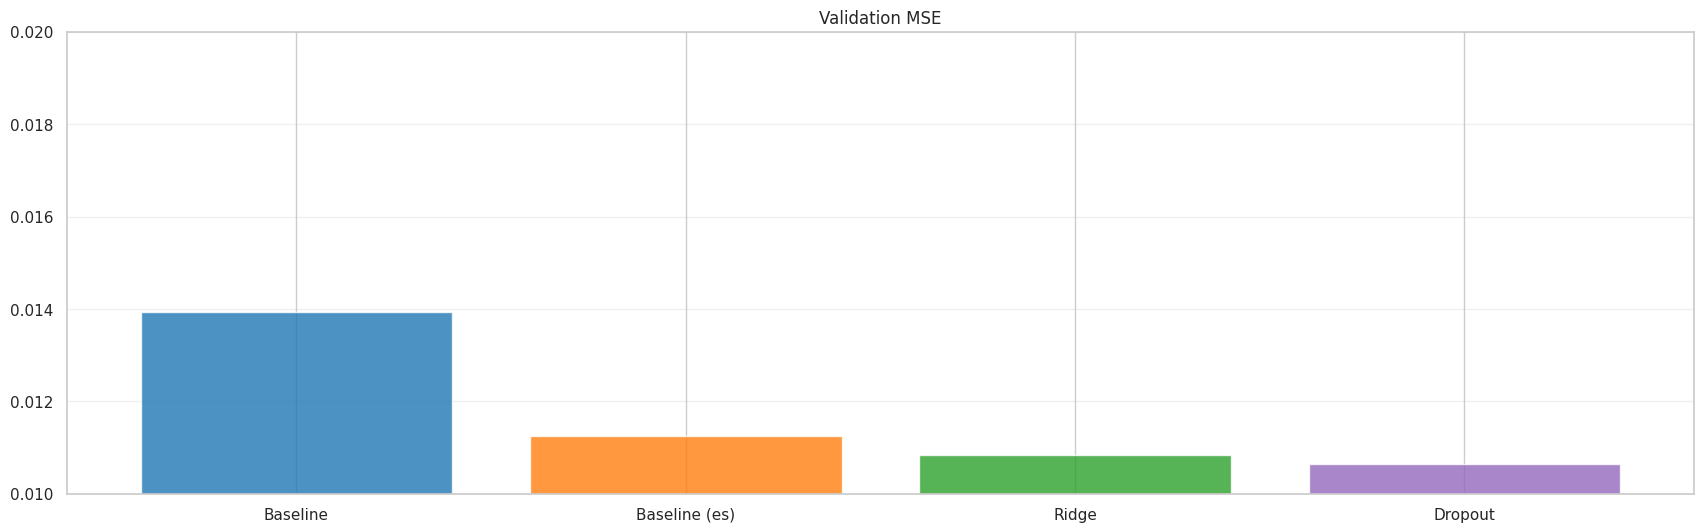
\includegraphics[width=1\textwidth]{Comparison2.png}
    \caption{Comparison of all methods}
    \label{fig:comparison2}
\end{figure}    

\end{document}